% ============================================================
% PRN232 - Section 5: Web Frontend (Vietnamese)
% ============================================================
\section{\bi{Cổng web Next.js 15}{The Next.js 15 Web Portal}}
\label{sec:web}

\subsection{\bi{Kiến trúc App Router}{App Router Architecture}}

\bi{
Cổng web được xây dựng bằng Next.js 15 với App Router, trên nền tảng
React 19 và Tailwind CSS với chủ đề ``Cinema Dark''. Kiến trúc App
Router thay thế mô hình \texttt{pages/} bằng cơ chế \emph{Server
Component} lồng nhau và \emph{Server Action}, cho phép dữ liệu được
lấy trực tiếp trên máy chủ mà không cần lớp API trung gian.
}{
The portal is built on Next.js 15 with the App Router, React 19 and
Tailwind CSS with a ``Cinema Dark'' theme. The App Router replaces the
\texttt{pages/} model with nested \emph{Server Components} and
\emph{Server Actions}, allowing data to be fetched directly on the
server without an intermediate API layer.
}

\begin{figure}[t]
\centering
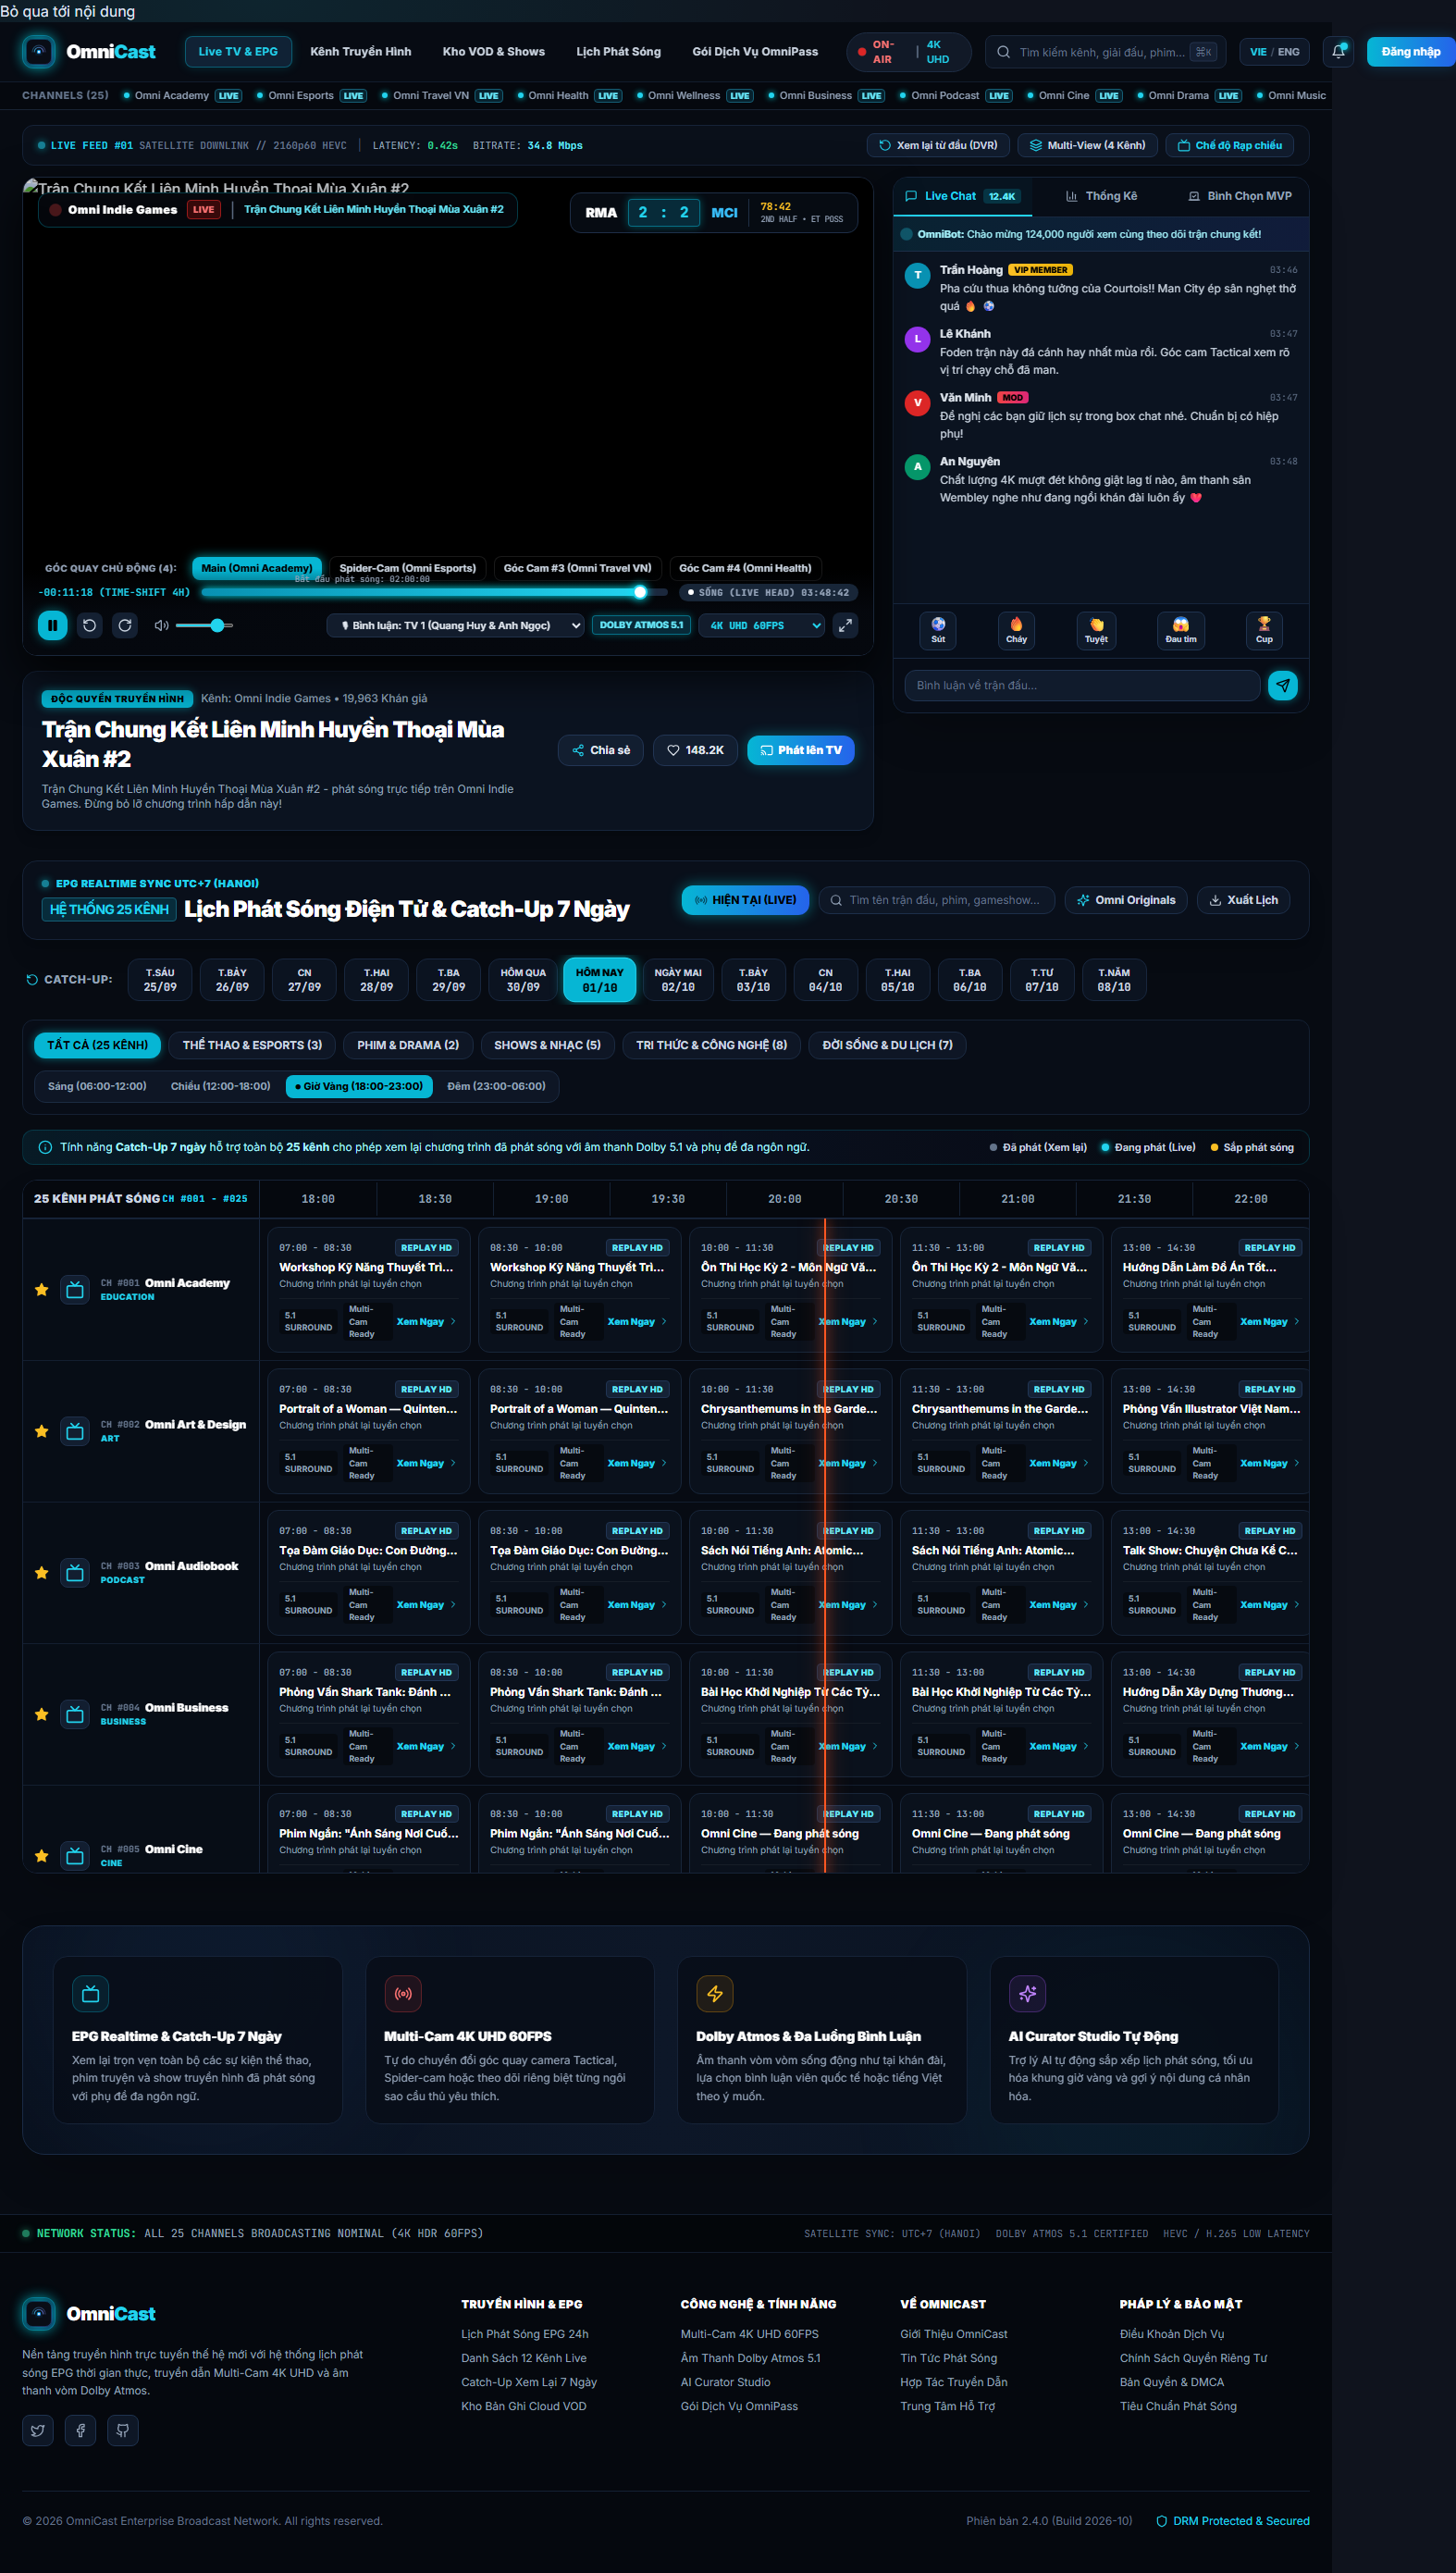
\includegraphics[width=\columnwidth]{../figures/01_home_desktop.png}
\caption{\bi{Trang chủ cổng web trên máy tính: carousel nổi bật, lưới
kênh theo thể loại và thanh điều hướng theo vai trò.}{The web portal
home page on desktop: featured carousel, channel grid by category and
the role-aware navigation bar.}}
\label{fig:home}
\end{figure}

\subsection{\bi{Cấu trúc route}{Route Structure}}

\bi{
Cổng web có 33 route được sinh từ 24 thư mục trong \texttt{app/}.
Các route được nhóm theo bốn nhóm chức năng: nội dung công khai
(\texttt{/}, \texttt{/channels}, \texttt{/epg}, \texttt{/programs},
\texttt{/recordings}, \texttt{/search}), xác thực và tài khoản
(\texttt{/login}, \texttt{/register}, \texttt{/forgot-password},
\texttt{/profile}, \texttt{/settings}), nghiệp vụ (\texttt{/live},
\texttt{/studio}, \texttt{/watchlist}, \texttt{/notifications}) và quản
trị (\texttt{/admin}, \texttt{/admin/users},
\texttt{/admin/audit-logs}). Ngoài ra còn có các trang tĩnh pháp lý và
hỗ trợ (\texttt{/terms}, \texttt{/privacy}, \texttt{/dmca},
\texttt{/standards}, \texttt{/broadcasting-standards}, \texttt{/help},
\texttt{/docs}).
}{
The portal exposes 33 routes generated from 24 folders under
\texttt{app/}. Routes fall into four functional groups: public
content (\texttt{/}, \texttt{/channels}, \texttt{/epg},
\texttt{/programs}, \texttt{/recordings}, \texttt{/search}),
authentication and account (\texttt{/login}, \texttt{/register},
\texttt{/forgot-password}, \texttt{/profile}, \texttt{/settings}),
business features (\texttt{/live}, \texttt{/studio},
\texttt{/watchlist}, \texttt{/notifications}) and administration
(\texttt{/admin}, \texttt{/admin/users},
\texttt{/admin/audit-logs}). Static legal and support pages
(\texttt{/terms}, \texttt{/privacy}, \texttt{/dmca},
\texttt{/standards}, \texttt{/broadcasting-standards}, \texttt{/help},
\texttt{/docs}) complete the list.
}

\begin{figure}[t]
\centering
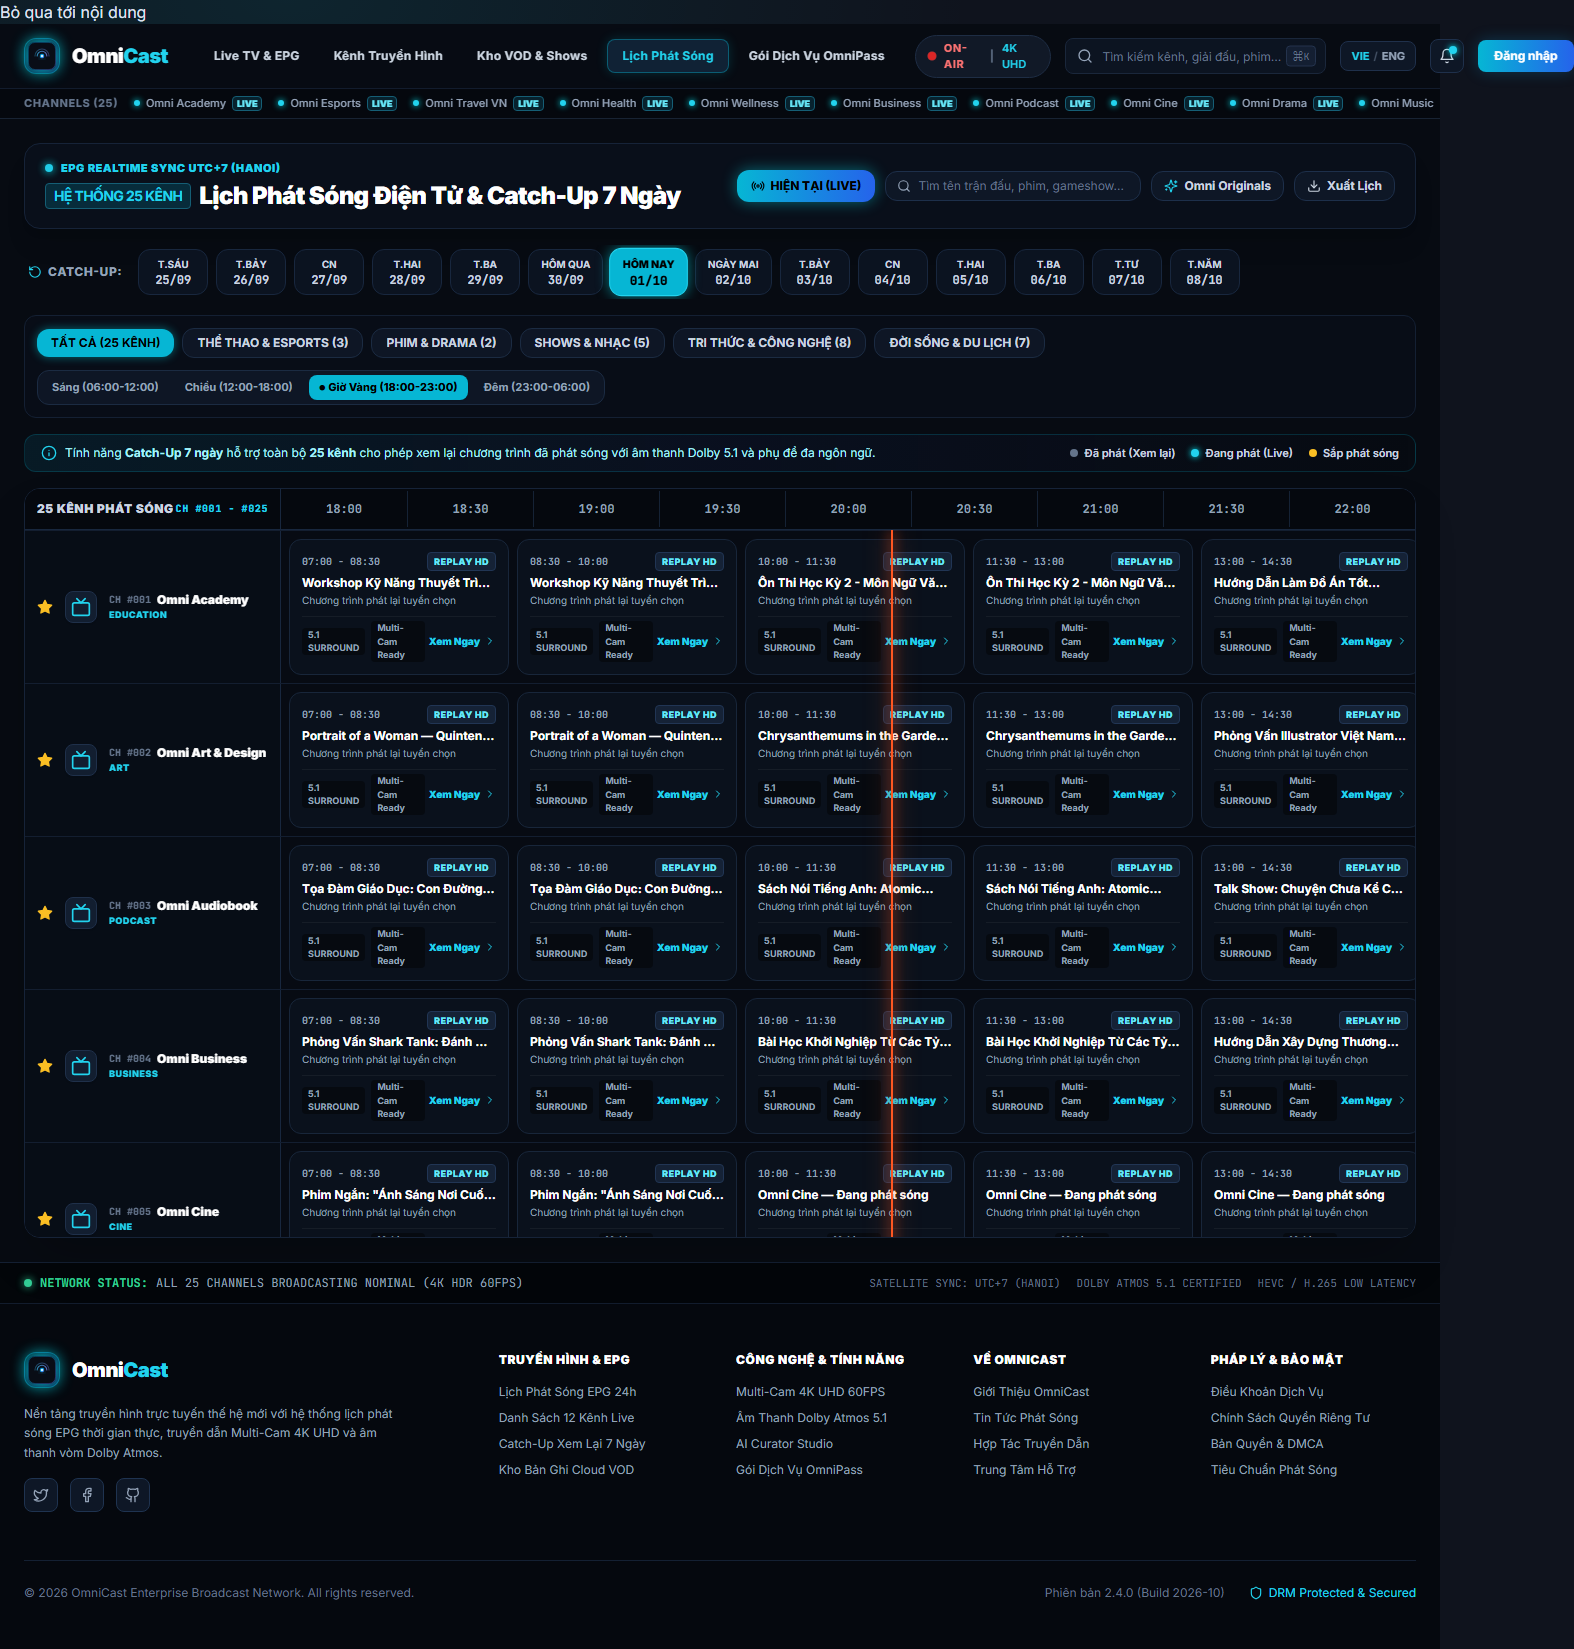
\includegraphics[width=\columnwidth]{../figures/subpage_epg.png}
\caption{\bi{Trang lịch phát điện tử với lưới theo khung giờ và bộ chọn
ngày.}{The electronic programme guide page with the time-slot grid and
the day selector.}}
\label{fig:epg}
\end{figure}

\subsection{\bi{Giao diện theo vai trò}{Role-Aware Interface}}

\bi{
Một tệp cấu hình duy nhất, \texttt{frontend/lib/constants/role-config.ts},
quyết định thành phần nào xuất hiện cho từng vai trò. Hàm
\texttt{hasMinimumRole} so sánh thứ hạng vai trò, nên việc nâng một
quyền từ \texttt{VIEWER} lên \texttt{STAFF} chỉ là sửa một dòng. Cùng
tệp này cũng khai báo tập icon Lucide đi kèm từng mục điều hướng, bảo
đảm điều hướng trên thanh đầu và chân trang luôn đồng bộ.
}{
A single configuration file,
\texttt{frontend/lib/constants/role-config.ts}, determines which
components appear for each role. The \texttt{hasMinimumRole} helper
compares role ranks, so promoting a capability from \texttt{VIEWER} to
\texttt{STAFF} is a one-line edit. The same file declares the Lucide
icon set accompanying each navigation entry, keeping the header and
footer navigation consistent.
}

\subsection{\bi{Các trang thành phần chính}{Key Component Pages}}

\bi{
Trang \texttt{/studio/curator} là giao diện biên tập AI: hiển thị danh
sách chương trình chờ duyệt, cho phép chạy lại quy trình AI, xem
điểm tin cậy, phân loại phù hợp phát sóng và các cảnh báo tuân thủ.
Trang \texttt{/studio/curator/audit} trình bày lịch sử các lần chạy
AI với dấu vết phiên bản prompt, cho phép so sánh kết quả giữa các
phiên bản. Trang \texttt{/studio/curator/dashboard} tổng hợp thống kê
phân bố theo thể loại, mức độ phù hợp phát sóng và tỉ lệ lỗi.
}{
The \texttt{/studio/curator} page is the AI curation interface: it
lists programmes awaiting review, allows re-running the AI pipeline,
and exposes the confidence score, broadcast-suitability classification
and compliance flags. The \texttt{/studio/curator/audit} page presents
the run history with prompt-version provenance so results can be
compared across revisions. The \texttt{/studio/curator/dashboard} page
aggregates statistics by category, broadcast-suitability and error
rate.
}

\begin{figure}[t]
\centering
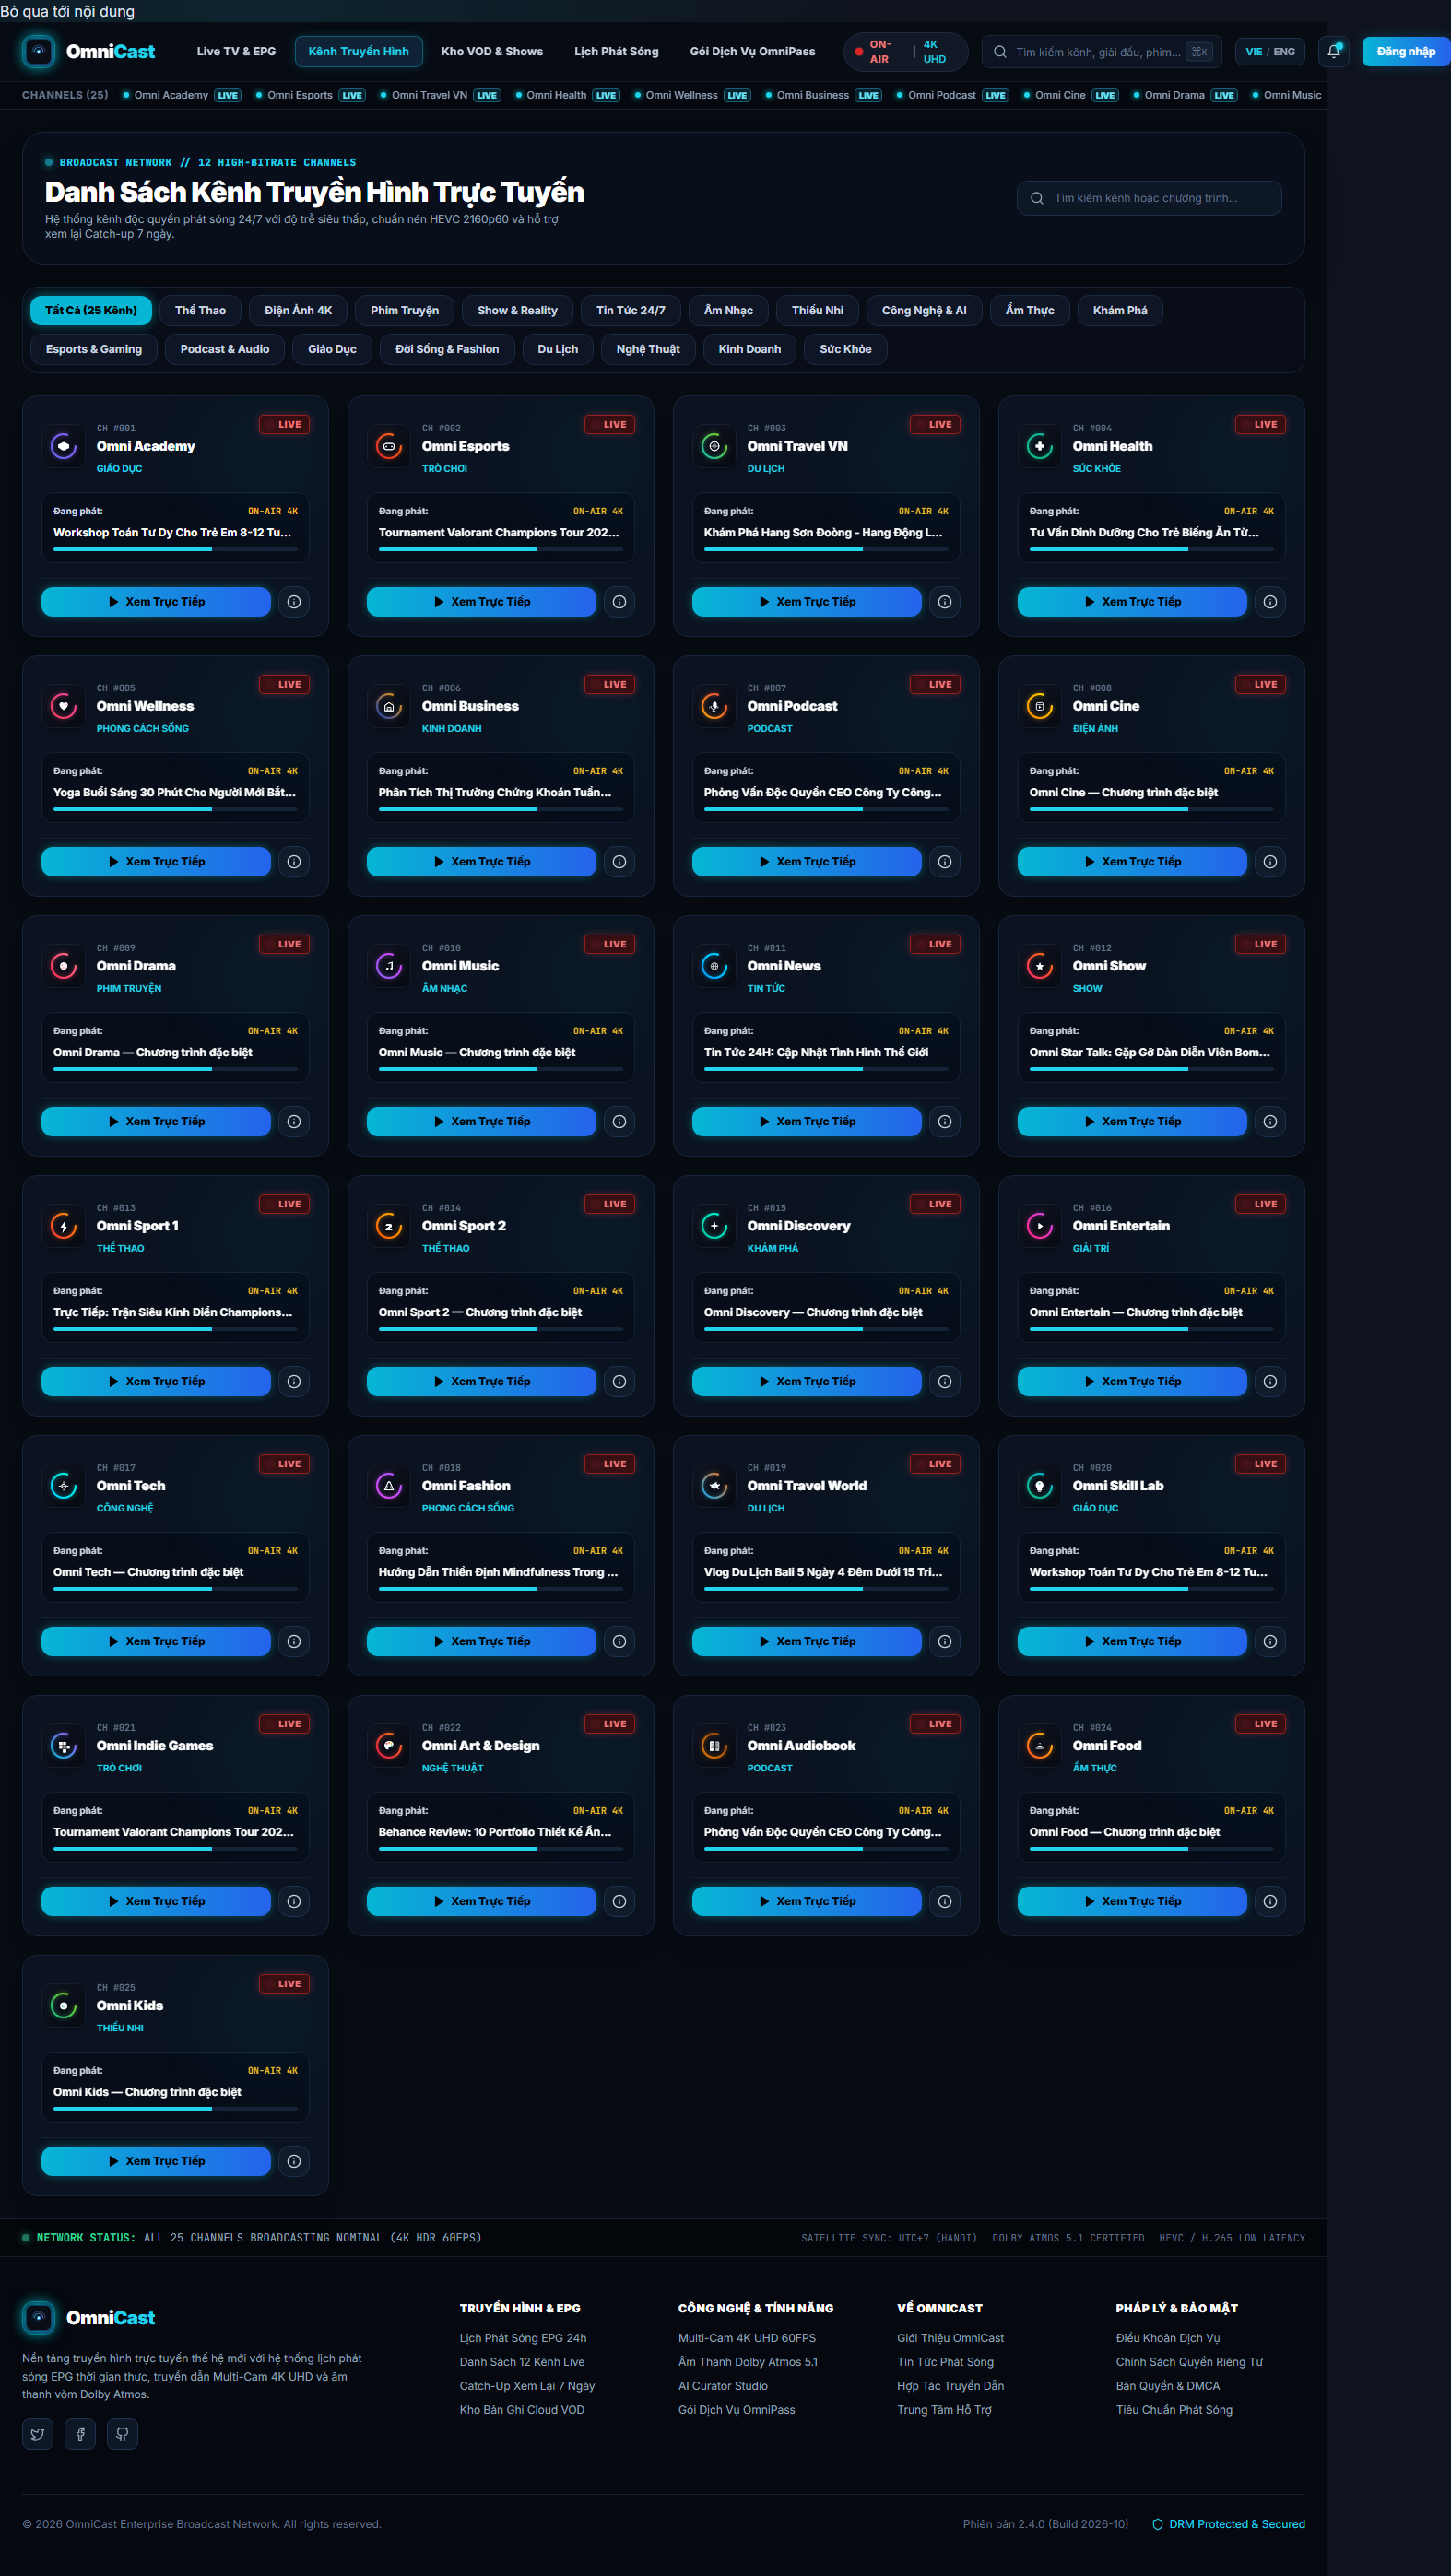
\includegraphics[width=\columnwidth]{../figures/subpage_channels.png}
\caption{\bi{Trang danh mục kênh với bộ lọc theo thể loại và thẻ nội
dung.}{The channel catalogue page with category filters and content
badges.}}
\label{fig:channels}
\end{figure}

\subsection{\bi{Bảo mật phía client và quản lý phiên}{Client-Side Security and Session Handling}}

\bi{
Cổng web dùng \texttt{next-themes} để hỗ trợ chế độ sáng/tối và một
lớp \texttt{safe-log} loại bỏ mọi dữ liệu nhạy cảm trước khi ghi log.
Mô đun \texttt{redact.ts} che các trường như mật khẩu, token và khoá
API; kiểm thử tương ứng trong \texttt{safe-log.test.ts} và
\texttt{redact.test.ts} bảo đảm hành vi che dữ liệu không bị hồi quy.
Khi người dùng đăng xuất, mọi phiên đăng nhập trên thiết bị khác được
thu hồi qua endpoint \texttt{logout-all}, tránh tình trạng phiên treo
sau khi đổi mật khẩu.
}{
The portal uses \texttt{next-themes} for light/dark support and a
\texttt{safe-log} layer that strips sensitive data before logging. The
\texttt{redact.ts} module masks fields such as passwords, tokens and
API keys; the corresponding tests in \texttt{safe-log.test.ts} and
\texttt{redact.test.ts} guard against regressions in that behaviour. On
logout, sessions on other devices are revoked through the
\texttt{logout-all} endpoint, preventing stale sessions after a
password change.
}

\subsection{\bi{Chất lượng mã nguồn và kiểm thử}{Code Quality and Testing}}

\bi{
Cổng web có 228 kiểm thử Vitest trong 76 bộ kiểm thử, bao phủ các hàm
thuần (\texttt{query-builder}, \texttt{curator-filters},
\texttt{curator-helpers}, \texttt{redact}, \texttt{safe-log},
\texttt{utils}), các hook (\texttt{useAiCurator},
\texttt{useAiCuratorStats}), các hàm cấu hình (\texttt{role-config}) và
các thành phần React (\texttt{video-player},
\texttt{save-to-watchlist}, các trang pháp lý, các trang studio).
CI còn chạy \texttt{tsc --noEmit} để bắt lỗi kiểu dữ liệu trước khi
biên dịch.
}{
The portal carries 228 Vitest tests across 76 suites, covering pure
functions (\texttt{query-builder}, \texttt{curator-filters},
\texttt{curator-helpers}, \texttt{redact}, \texttt{safe-log},
\texttt{utils}), hooks (\texttt{useAiCurator},
\texttt{useAiCuratorStats}), configuration (\texttt{role-config}) and
React components (\texttt{video-player}, \texttt{save-to-watchlist},
the legal pages, the studio pages). CI additionally runs
\texttt{tsc --noEmit} to catch type errors before the build.
}
